\section{Related Work}
\subsection{Malware Analysis}
Malware analysis is a critical aspect of cybersecurity, enabling the identification
and mitigation of malicious software threats.
Analysis techniques can be roughly categorized into two classes: static and dynamic.

\subsubsection{Static Analysis}
Static analysis involves examining the structure and content of a suspected malicious file without executing it.
Static analysis are often conducted as a preliminary step to grasp the general characteristics of the malware
before more sophisticated analysis techniques are applied \cite{chakkaravarthy2019survey}.

\textbf{Signature matching} is a common technique that compares the "signature", characteristics of a file
against a database of malware such as VirusTotal \cite{VirusTot28:online}. The characteristics include file size, hash values, and byte sequences.
Although this method has been a staple in malware detection, it is limited by its inability to detect only known malware.

\textbf{Disassemble and decompile} is another static analysis technique
that involves converting the binary code of a malware into a human-readable format.
From the decompiled code, analysts might be able to identify the malware's functionality and behavior as well as finding
interesting strings like URLs, IP addresses, and encryption keys.

\subsection{Dynamic Analysis \cite{10.1145/3329786}}
Dynamic analysis entails examining the behavior of malware by executing it in a controlled environment.
This approach enables analysts to witness the interactions between the malware and the system,
providing insights into its true intentions and capabilities.

\textbf{Function call analysis} is a method that focuses on tracking functions issued by the malware and the parameters
passed to them. One way to archive this is by code injection, in which analyzing code is hooked into
a specific function call and various information is collected and notified when the function is called.
Carsten et al. \cite{willems2007toward} created an automated malware analysis system that injects DLLs within CWSandbox,
letting analysts monitor system calls.

\textbf{Data flow tracking} is another approach that tracks the flow of data through the malware, and data tainting is an established
technique in this area. It involves marking (or "tainting") specific data components and then monitoring
how this tainted data propagates through the system.
Data tainting could be utilized in static analysis, but due to some evasion strategies like encryption and obfuscation
it has endured challenges in practice \cite{alashjee2019dynamic}.
SELECTIVETAINT \cite{chen2021selectivetaint} was invented to address performance overhead issue by employing static binary
rewriting to selectively instrument only instructions related to taint analysis.


\subsection{Shadow Attack \cite{Weiqin:ShadowAttack}}
Shadow Attack is one of the techniques used by malware writers to evade behavior-based detection systems,
orchestrating multiple processes to stealthily carry out malicious activities.

Such detectors typically rely on comparing system call graph within a process under scrutiny with predefined
malware specifications established on specific sequences or graphs of system calls\cite{inproceedings}.
For example, the malware specification of download-and-execute is expressed as follows \cite{Weiqin:ShadowAttack}:
\begin{equation}
  \texttt{recv} \land \texttt{open} \rightarrow \texttt{write} \rightarrow \texttt{exec}
\end{equation}
, where $s_1 \land s_2$ denotes both of two system calls $s_1, s_2$ are executed and $s_1 \rightarrow s_2$
denotes $s_1$ is followed by $s_2$.

So more specifically, the goal of Shadow Attack is to bypass dynamic malware detection based on
the analysis of system call graphs by exporting any critical system call included in malware specifications to
other collaborating processes, which is called shadow processes.
We call the Communication shadow processes do with each other as Shadow Process Communication (SPC).
The concept of Shadow Attack is illustrated in \Fref{img:shadow-attack}.
\begin{figure}[tp]
  \begin{center}
    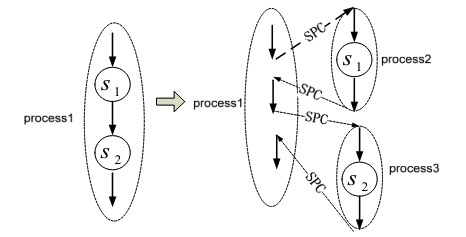
\includegraphics[width=\columnwidth]{./img/archi_SA.png}
  \end{center}
  \caption{Illustration of Shadow Attacks
    \cite{Weiqin:ShadowAttack}}
  \label{img:shadow-attack}
\end{figure}

Shadow attacks can be categorized into in-host, remote-network-coordinated, and hybrid.
In in-host shadow attacks, all shadow processes are executed on the same host and SPCs are conducted through
unix domain socket or stream pipe, while remote-network-coordinated shadow attacks involve multiple remote hosts
that are connected through network sockets.
Prototype implementation is made by the authors only for in-host shadow attacks.

One countermeasure is extracting correlation between processes and reconstructing
the original system call graph, but the authors conducted an evaluation experiment following this approach,
whose result suggested that solution would encounter challenges of high overhead.

\subsection{eBPF}
\subsubsection{Berkeley Packet Filter}
Steven and Van \cite{mccanne1993bsd} proposed the BSD Packet Filter architecture in 1993 for efficient packet capture on
Unix-based operating systems. In the following, we refer to Berkeley Packet Filter as "BPF."
At the time of paper publication, packet capture involved copying all packets acquired in the kernel
space to the user space before filtering.
This process resulted in unnecessary overhead. \cite{mccanne1993bsd} devised a pseudo-machine (BPF pseudo-machine)
that interprets programs written in special 32-bit instructions to perform filtering.
By running this pseudo-machine in the kernel space, they addressed the issue. Compared to existing systems,
BPF operated up to 20 times faster.
The overview of BPF architecture is shown in Figure \ref{img:bpf_old}.

BPF was introduced in the Linux kernel as "Linux Socket Filter" in version 2.1.75 and
was used to accelerate the \texttt{tcpdump} command.

\subsubsection{Extended Berkeley Packet Filter}
BPF underwent significant improvements and extensions in the Linux kernel version 3.18,
leading to the emergence of extended BPF, commonly referred to as eBPF \cite{Linux31836:online}.
The enhancements cover various aspects, with notable additions summarized below \cite{learning-ebpf}:
\begin{itemize}
  \item 64-Bit BPF Instruction Set: The BPF instruction set was reworked from 32-bit to 64-bit, resulting in improved execution efficiency.
  \item eBPF Maps: The introduction of eBPF maps allowed data sharing between user space and kernel space. These maps serve as a mechanism for efficient communication.
  \item eBPF Verifier: To ensure safe execution of eBPF programs, an eBPF verifier was added. It validates the correctness and security of eBPF code.
\end{itemize}

\begin{figure}[tp]
  \begin{center}
    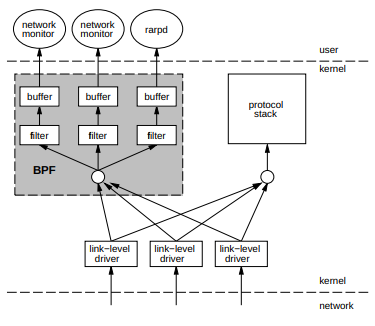
\includegraphics[width=\columnwidth]{./img/bpf_overview.png}
  \end{center}
  \caption{The overview of BPF architecture. It accelerates packet capture
    by performing filtering in the kernel space. \cite{mccanne1993bsd}}
  \label{img:bpf_old}
\end{figure}

The area covered by eBPF has also expanded.
In the context of networking, it has become able to handle various layers of the Linux network stack,
such as unix domain sockets and network devices.
Additionally, eBPF programs can now be used for performance tracing and enhancing the security of Linux systems,
leading to the term "BPF" losing its original meaning of "Berkeley Packet Filter" and being used as an independent term.

For convenience, BPF before the extension in v3.18 is sometimes referred to as classical BPF or cBPF.

\subsection{Overview of eBPF Architecture}
An overview of the eBPF architecture is shown in \Fref{img:ebpf-system}.
Hereafter, we describe the important processing flows with reference to \Fref{img:ebpf-system}.
\begin{figure}[tp]
  \begin{center}
    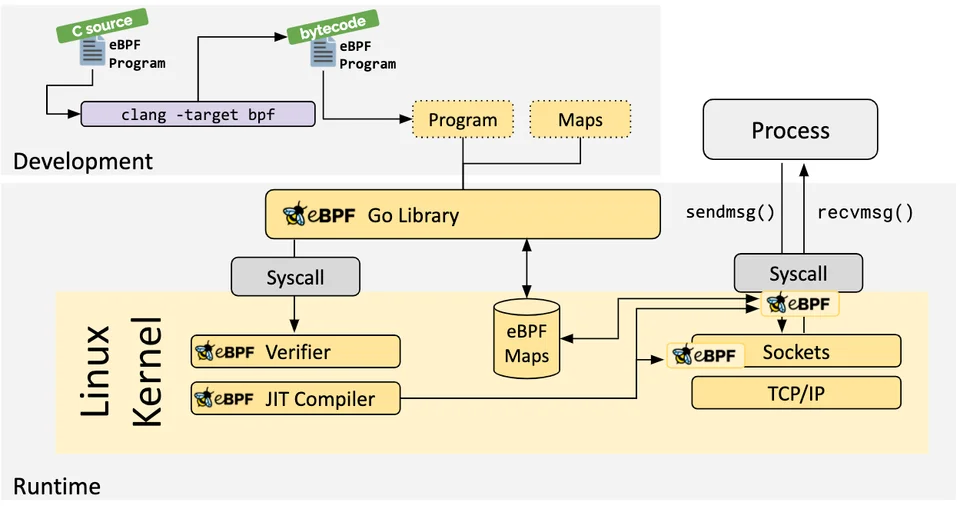
\includegraphics[width=\columnwidth]{./img/ebpf_system.png}
  \end{center}
  \caption{The overview of eBPF architecture. This figure shows how eBPF programs are compiled, verified, and executed.
    \cite{WhatiseB29:online}}
  \label{img:ebpf-system}
\end{figure}

\subsubsection{Event-Driven Architecture}

eBPF has an event-driven architecture.
The mechanism involves hooking an eBPF program to an event in the kernel, and then
performing the specified processing when the event occurs. eBPF programs can be dynamically loaded or removed.

The events that eBPF can hook into are defined as Program Types in the kernel's source code \footnote{\texttt{include/uapi/linux/bpf.h}}.
A few examples of Program Types are as follows:
\begin{itemize}
  \item XDP: An event for manipulating packets before data is copied to the kernel space when a packet arrives at a network device.
  \item Tracing: An event for detecting kernel function calls and passing tracepoints.
  \item LSM: An event for applying security policies using the Linux Security Module.
\end{itemize}
When such events occur, the eBPF program executes the processing corresponding to the Program Type.
For example, a program hooked to an XDP event can decide whether to accept or drop a packet.

\subsubsection{eBPF Verifier}
The eBPF verifier is a program that takes eBPF programs converted to bytecode as input and
verifies that they can be executed safely on the kernel.
The bytecode is loaded into the kernel via the \texttt{bpf()} system call
(shown as "Syscall" in \Fref{img:ebpf-system}), but the program will not run unless it passes verification by the verifier.
Specifically, it checks for things like avoiding memory access violations, ensuring the program exits normally,
and that the program is not granted unnecessary privileges.

In this way, the eBPF verifier enhances security by imposing restrictions on eBPF programs.
Since the verifier plays a crucial role in eBPF,
research has been conducted to mathematically verify the logic of the verifier \cite{vishwanathan2023verifying}.

\subsubsection{JIT Compilation}
The eBPF bytecode that passes the verifier is converted by a JIT compiler into machine code
that directly runs on the target CPU. This optimizes the execution speed, allowing it
to operate as efficiently as the kernel and kernel modules directly compiled from source code
\cite{WhatiseB29:online}.

\subsubsection{Kernel Modules}
Kernel modules are a mechanism that allows for the extension of kernel functions without modifying the kernel's
source code by loading object files during the execution of the Linux kernel.
Kernel modules are not subject to constraints like the eBPF verifier, thus offering a high degree of program freedom.
However, since kernel modules are executed with the same privileges as the kernel,
it is necessary to develop carefully to avoid embedding vulnerabilities \cite{chen2011linux}.

As Mayer et al. \cite{mayer2021performance} point out, avoiding the creation of kernel modules can be
considered an advantage of eBPF.
